\chapter{Abweichungen der Fitting-Plots}
\begin{table}[h]
    \centering\begin{tabular}{cc}
      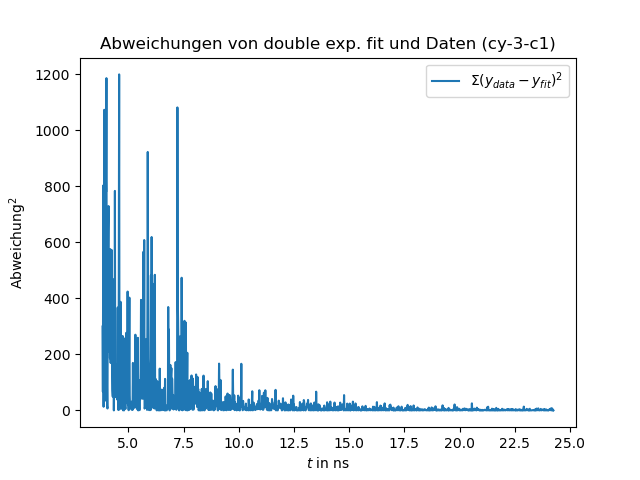
\includegraphics[width=0.45\textwidth]{Anhang/Fit/def31.png} & 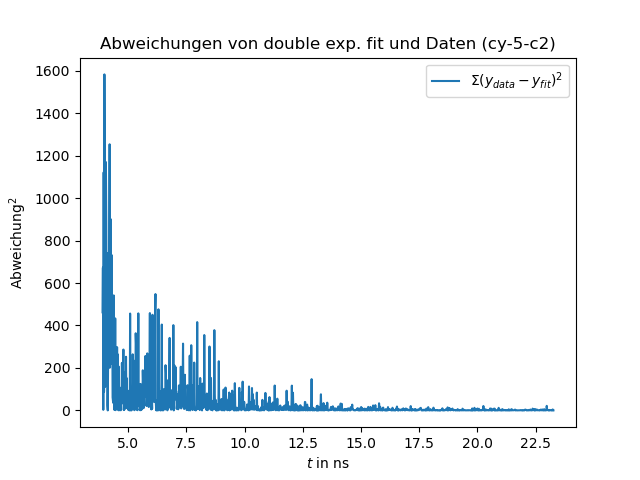
\includegraphics[width=0.45\textwidth]{Anhang/Fit/def52.png}\\
      Double exp fit und Daten (cy-3-c1) & Double exp fit und Daten (cy-5-c2)\\
      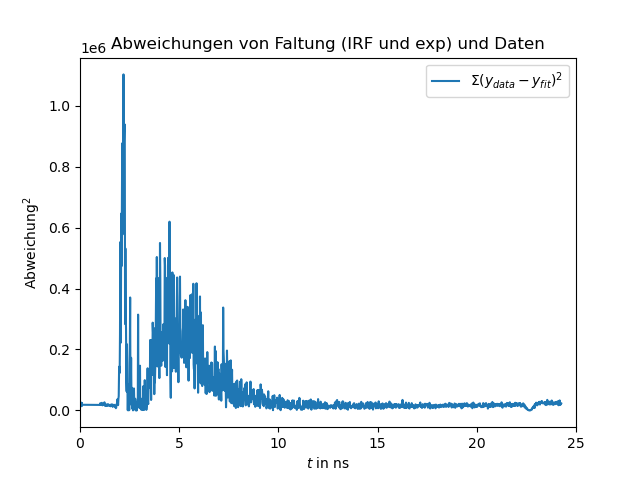
\includegraphics[width=0.45\textwidth]{Anhang/Fit/afd.png} & 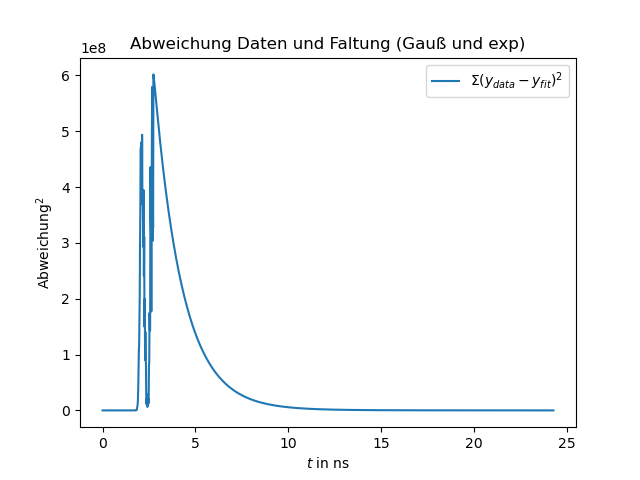
\includegraphics[width=0.45\textwidth]{Anhang/Fit/agfd.png}\\
      Faltung und Daten & Gauss-Faltung und Daten
    \end{tabular}
    \caption{Abweichungen der Fits}
  \end{table}